%!TEX root = thesis_main.tex

\chapter{Single-Stage Cycloid Design}\label{ch:design_1s}

%Intro to the chapter here. Talk about what I talked about, basically a Chapter 2 abstract 
Single-stage cycloidal drives have been relatively well studied in theory regarding their profiles, machining considerations, load estimates, and simulation results. However, two gaps in the literature have been identified. The first is in the actual in-use efficiency and lifetime characteristics of a single-stage cycloid. The second is a more rigorous definition of the relative motion between the cycloid plate and the housing pins to further characterize losses in the system. This chapter will first cover the theoretical profile generation of the cycloid plates in section \ref{ch:design:basic_calc}. Next, the new calculations for the relative motion and associated losses for the interactions between the single-stage cycloid plate pins and rollers are detailed in Section \ref{ch:design:pin_roll_1s}. Finally, the design of the single-stage cycloid that was tested is reviewed in Section \ref{ch:design:single}.

\section{General Design Calculations} \label{ch:design:basic_calc}
% Talk about the basic design equations for a cycloid, how do you generate the driving profile? 

Cycloidal drives harness a unique motion to create the desired reduction ratios in an actuator. The combination of an eccentric input coupled with an epitrochoid plate creates a potentially high reduction device. In addition, this device is made of solid, relatively easy to manufacture pieces, giving it a unique advantage over other high reduction systems such as a harmonic drive in its ease of manufacturing and capability to withstand shock loads. The design equations for many aspects of a single-stage cycloidal design have been well covered in the literature. The basic generating profiles will be discussed here to develop an understanding of the motion to lay a foundation for additional analysis and calculations for a single-stage design in Section \ref{ch:design:pin_roll_1s}, and as a basis for a two-stage design presented in Chapter \ref{ch:single}. 

\subsection{Conceptual Overview of Cycloidal Motion} \label{ch:design:basic_calc:overview}

Cycloidal drives utilize eccentric motion to induce interactions between the cycloid plate and housing rollers. This creates a counter-rotation that is harnessed as the transmission's output. The basic construction of a single-stage cycloid can be seen in Figure \ref{fig:single_cartoon} and involves four distinct pieces
\begin{enumerate}
	\item the motor input, a concentric shaft with an eccentric circle with eccentricity \textit{E} (gray);
	\item the ``cycloid plate'' that is mounted to the eccentric circle (blue);
	\item the housing that contains the rollers that the cycloid plate interacts with (yellow); and
	\item the output, which uses pins to harness the rotation of the cycloid plate and bring the motion back to concentric (orange).
\end{enumerate}

\begin{figure}[t]
   \centering
   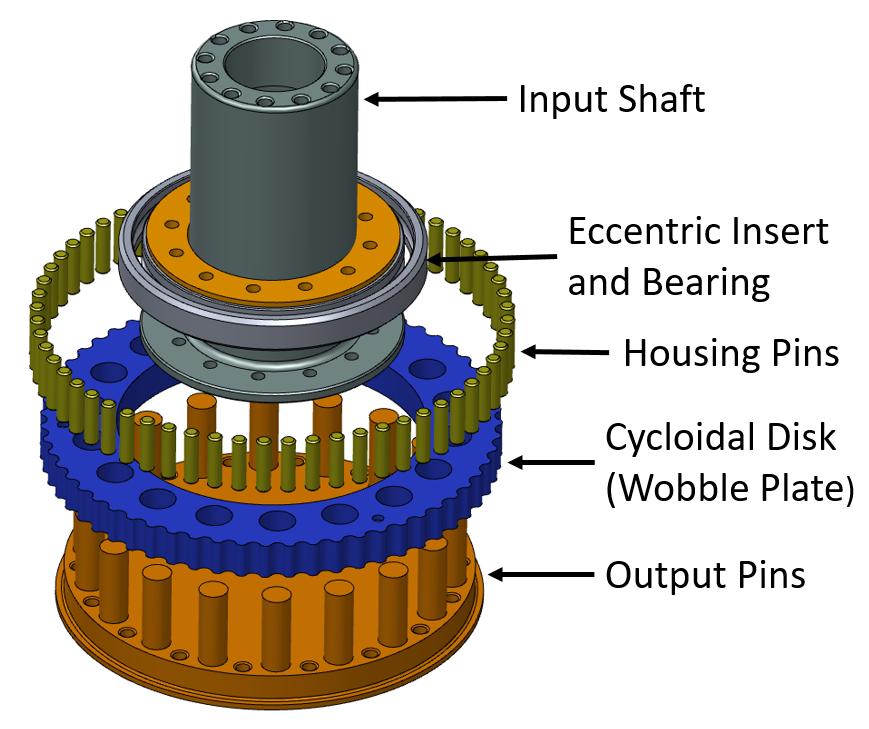
\includegraphics[width=0.60\linewidth]{fig/cycloid_cartoon_v2}
   \caption{Simple rendering of the key elements that create a cycloidal drive.
   A drive shaft spins a cycloidal plate via an eccentric circle.
   The cycloid plate reacts against the housing pins to create a counter-rotation, harnessed by the output pins.}
   \label{fig:single_cartoon}
\end{figure}
%\todo[inline]{change cycloid disk to cycloid plate in figure}

The motion induced is complex and generally non-intuitive. An illustration of this motion can be seen in the collection of images in Fig. \ref{fig:single_motion}. The system is designed such that the cycloid plate has one fewer lobe than the housing has rollers \cite{ref:pollitt}. Analysis has been done on systems with more than one lobe difference \cite{ref:hsieh_traditional}, but a single lobe difference is used in this work. If the housing did not exist, the cycloid plate would just move in an eccentric circle with no rotation due to the input shaft's eccentricity. However, due to the lobes interacting with the pins in the housing, and there being one fewer lobes than pins, the lobes move into the spaces between the pins during the eccentric motion. The pushing of the cycloid plate lobes into these gaps causes the cycloid plate to rotate about it's local axis, which will be referred to as the C-axis. This counter-rotation is defined by equation \ref{eq:single_stage_ratio_2} \cite{ref:on_the_lobe} where \textit{N\textsubscript{1}} is the number of housing rollers.

\begin{figure}[t]
   \centering
   \begin{tabular}{cccc}
     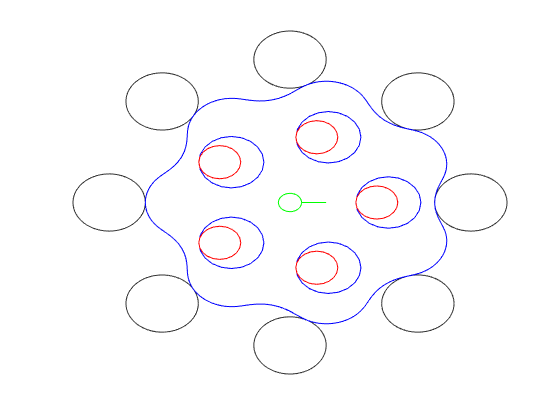
\includegraphics[width=0.24\linewidth]{fig/single_0} &
     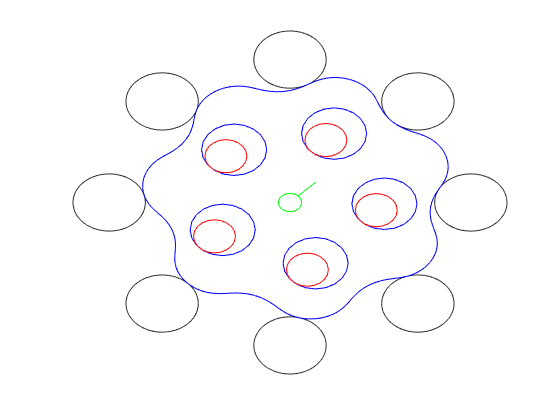
\includegraphics[width=0.24\linewidth]{fig/single_1} &
     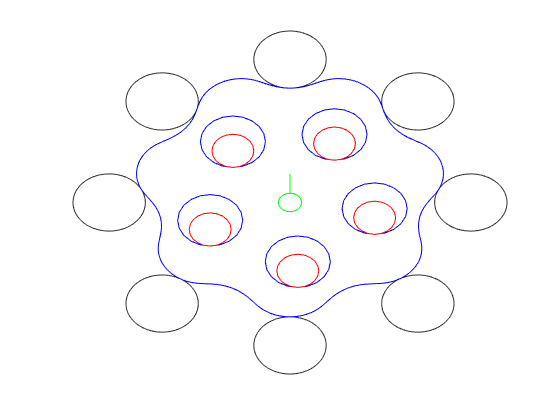
\includegraphics[width=0.24\linewidth]{fig/single_2} &
     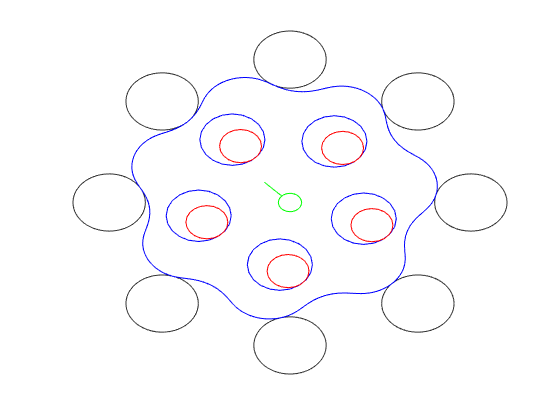
\includegraphics[width=0.24\linewidth]{fig/single_3} \\
     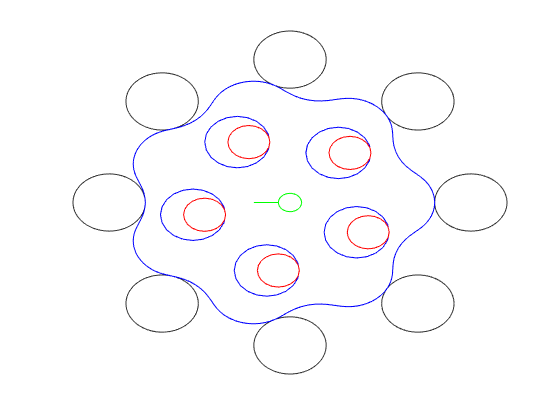
\includegraphics[width=0.24\linewidth]{fig/single_4} &
     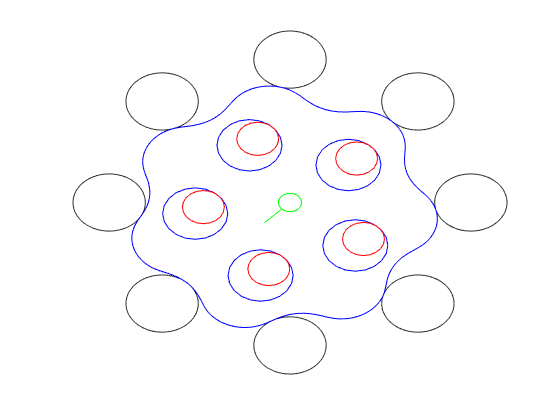
\includegraphics[width=0.24\linewidth]{fig/single_5} &
     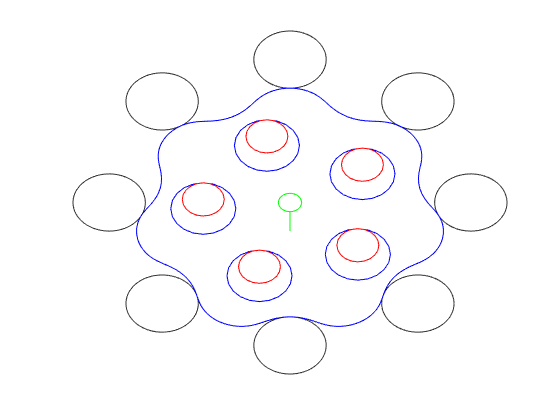
\includegraphics[width=0.24\linewidth]{fig/single_6} &
     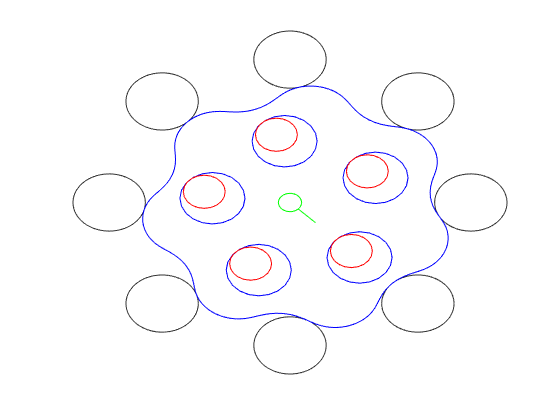
\includegraphics[width=0.24\linewidth]{fig/single_7} \\
   \end{tabular}
   \caption{An example of a single-stage cycloid motion with eight pins (black), seven lobes (blue) for a ratio of 7:1 and five output pins (red) for one full input rotation resulting in 1/7 counter-rotation of the cycloid plate.}
   \label{fig:single_motion}
\end{figure}

\begin{equation} \label{eq:single_stage_ratio_2}
Q = \frac{N_1-1} {N_1 - (N_1 - 1)} = N_1 -1
\end{equation}

The intuition for the creation of the counter-rotation of the cycloid plate has now been established, but this counter-rotation must be harnessed in order to create an effective reduction. This is where the output pins play in. The output must not only harness the counter-rotation but must also return the output to be concentric with the input to be used effectively. If the output were fixed to the cycloid plate, the output would have eccentric motion. This results in the conceptual design presented, in which an output plate is mounted on a concentric bearing and has pins of radius \textit{R\textsubscript{o}} that are fixed to it. These pins insert into the cycloid plate into holes that are of diameter $R_{hole}$.

\begin{equation} \label{eq:pin_hole_diam}
R_{hole} = R_o + E.
\end{equation}

This larger diameter hole allows the cycloid plate to move eccentrically around the pins. Therefore, half of the pins are receiving the load at any one time from the cycloid plate. This concept allows for the compact high reductions and loads seen in single-stage cycloids. 

\subsection{Lobe Profile Calculation} \label{ch:design:basic_calc:profile}

Now that the basic design and motion of a single-stage cycloid has been established, the specific profile that allows the meshing of the cycloid plate with the housing pins can be discussed. These equations have been presented by multiple authors in previous works; however, they will be fully described in this section to allow expansion upon later chapters. 

\begin{figure}[!b]
   \centering
   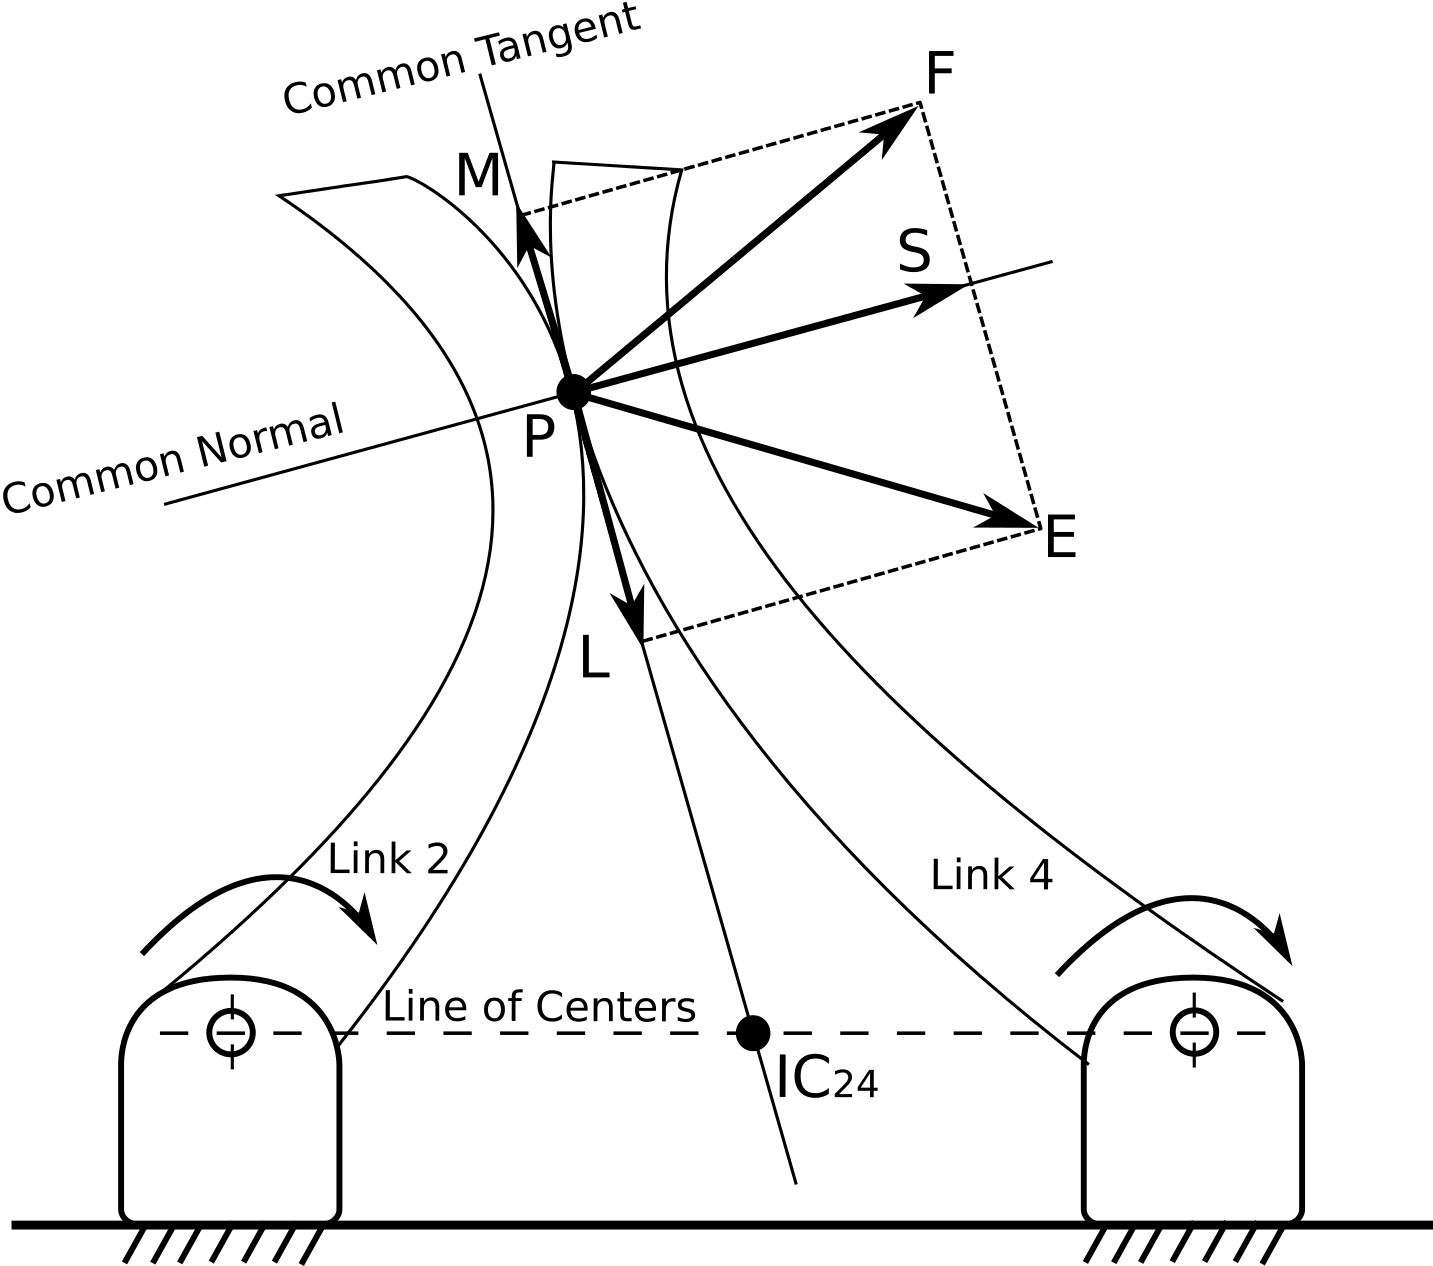
\includegraphics[width=0.60\linewidth]{fig/kennedy_sliding}
   \caption{Graphical articulation of Kennedy's Theorem. The contact points on Link 2 and 4 have their own velocity, \textit{F} and \textit{E}, determined by their own motion. However, to remain in contact, their respectively velocities in the \textit{S} direction must be equal. The remaining motion, along the common tangent \textit{M} and \textit{L} respectively indicates the relative sliding between the links. In additional, the instant center of Links 2 and 4, by Kenney's Theorem, must lie along the \textit{Line of Centers} of the two link's rotation. (This figure was adapted from \cite{ref:kinematics_and_dynamics})}
   \label{fig:kennedy_sliding}
\end{figure}

The work by Shin et. al. \cite{ref:on_the_lobe} describes the generating equations for the cycloid profile well and was the basis for the equations used in this work. However, many other works prior to Shin et. al. give the full detail of these profiles \cite{ref:malhorta_2}, \cite{ref:hwang_hsieh}, \cite{ref:design_and_application}.
The cycloid plate profile, if manufactured perfectly, would result in the lobes of the cycloid plate staying in perfect contact with the housing pins throughout the motion. In practice, some clearance is desired when not transmitting load to allow assembly and manufacturing tolerances. The basic principle that is harnessed to generate these profiles is Kennedy's Theorem. Kennedy's Theorem states that ``any three bodies having planar motion relative to one another have three instant centers, and they lie on a straight line''\cite{ref:kinematics_and_dynamics}.  That is, any two bodies that are in contact must have an instant center that falls along the line made by the line of centers of the bodies. In addition, this instant center must also fall along the common tangent line of their interaction. This concept is illustrated in Figure \ref{fig:kennedy_sliding}. Using this definition for where the instant center falls for the contact between the bodies and the common normal, the equations for the profile to meet these criteria can be generated. 

Before the equations are defined, a number of parameters necessary for design must be established. These parameters are listed in Table \ref{table:variable_definitions}. 
The design parameter decisions and restrictions for the tested actuator will be discussed further in section \ref{ch:design:single}. 

\begin{table*}[!b]
  \vskip0.2cm
  \caption{Design Variables}
  \label{table:variable_definitions}
  \begin{center}
    \vskip-0.2cm
    \begin{tabular}{|p{0.14\textwidth}|p{0.40\textwidth}|}
    \hline
    Variable Designation & Variable Description\\
    \hline
    \hline
    \textit{E} & eccentric offset distance\\
    \hline
    \textit{R\textsubscript{r}} & radius of the housing roller \\
    \hline
    \textit{R} & radius from the fixed frame center to the center of the housing roller\\
     \hline
    \textit{R\textsubscript{ro}} & output pin diameter \\
     \hline
    \textit{N\textsubscript{1}} & number of housing rollers \\
     \hline
    \textit{N\textsubscript{o}} & number of output pins\\
     \hline
    \textit{\textphi\textsubscript{2}} & the input angle from the motor \\
     \hline
    \textit{\textphi\textsubscript{3}} & the output angle of the cycloid plate \\
    \hline
    \end{tabular}
  \end{center}
\end{table*}

With these defined parameters, the equations necessary for generating the profiles can be developed.
Figure \ref{fig:single_frames} shows an illustration of the frames necessary for a single-stage cycloid. In this case, the first link is the ground link, the second link is the motor input via the eccentric arm, and the third link is the cycloid plate itself. The interaction that must satisfy Kennedy's Theorem is between the cycloid link and the ground link (links 1 and 3). The interaction between those two links must have an instant center that falls on the line of instant centers I\textsubscript{12} and I\textsubscript{23} that is normal to the common tangent. To create the cycloid plate profile, the location of this point must be put into the frame of the cycloid plate. Three frames are denoted in Figure \ref{fig:single_frames}, the fixed frame \textit{F}, the motor frame \textit{M}, and the cycloid plate \textit{C}. 

\begin{figure}[!b]
   \centering
   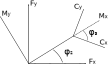
\includegraphics[width=0.50\linewidth]{fig/single_stage_frames}
   \caption{Coordinate frames used to compute the rotation matrices for cycloid plate profile generation.}
   \label{fig:single_frames}
\end{figure}
\todo[inline]{fix frames to show Cx}

The transforms between the fixed frame and the motor frame (Eq. \ref{eq:T_fm}) and the motor frame and the cycloid frame (Eq. \ref{eq:T_mc}) are first defined. 

\begin{equation} \label{eq:T_fm}
T_f^m = \left[{\begin{array}{cccc}
		cos(\phi_2) & -sin(\phi_2) & 0 & 0\\
		sin(\phi_2) & cos(\phi_2) & 0 & 0\\
		0 & 0 & 1 & 0\\
		0 & 0 & 0 & 1 \end{array} } \right]
\end{equation}

\begin{equation} \label{eq:T_mc}
T_m^c = \left[{\begin{array}{cccc}
		cos(\phi_2 - \phi_3) & -sin(\phi_2 - \phi_3) & 0 & E\\
		sin(\phi_2 - \phi_3) & cos(\phi_2 - \phi_3) & 0 & 0\\
		0 & 0 & 1 & 0\\
		0 & 0 & 0 & 1 \end{array} } \right]
\end{equation}

Next, the point of intersection, \textit{P}, between links 1 (the ground via the housing roller) and link 3 (the cycloid plate) can be defined using the Figure \ref{fig:single_angles}. The line between the two centers of rotation for the motor (link 1 to link 2) and the cycloid plate (link 2 to link 3) is extended and shown as a dotted line. A line is then drawn from the center of the housing roller to the intersection of the extended line of centers and the intersection is labeled \textit{M}. The length of OM can be defined as \textit{EN\textsubscript{1}} in \cite{ref:on_the_lobe}. This defines the common normal line to the common tangent of interaction between the housing roller and the cycloid plate. Therefore, triangles can be drawn, and using this definition the angle, \textpsi,\ can be found. 

\begin{equation} \label{eq:psi}
\psi = \tan^{-1}{\bigg\{\frac{\sin\phi_2}{\frac{R}{EN} - \cos{\phi_2}}\bigg\}}
\end{equation}

The location of point P with respect to the fixed frame can then be defined as 

\begin{equation} \label{eq:Cf}
C_f = \left[\begin{array}{c}
		R-Rr*cos(\psi)\\
		Rr*sin(\psi)\\
		0\\
		1
		\end{array} \right]
\end{equation}


\begin{figure}[t]
   \centering
   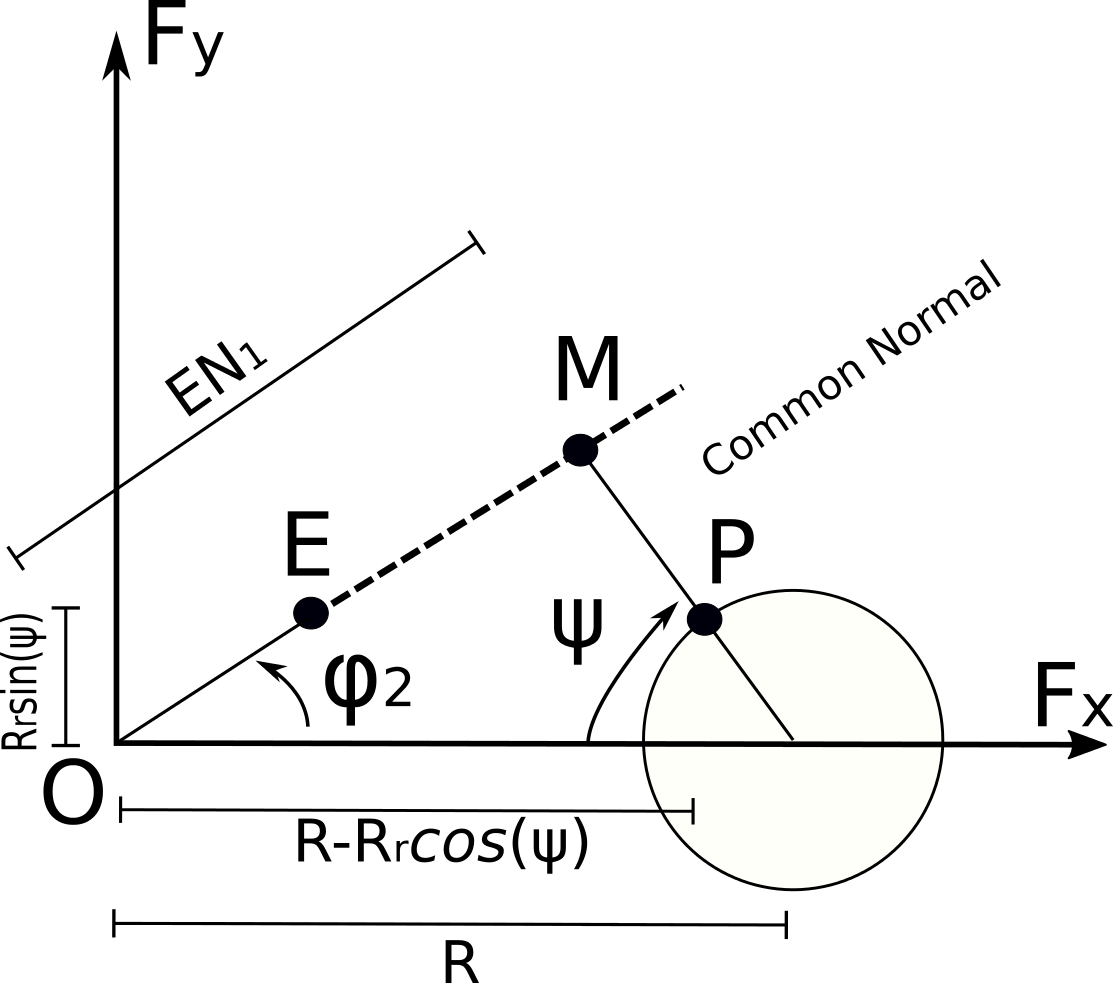
\includegraphics[width=0.60\linewidth]{fig/single_stage_angles}
   \caption{Depiction of the interaction between the three links, the ground link that includes the housing pin, the motor link OE, and the cycloid link EP. The line of centers is drawn between the motor to ground connection at O and the cycloid plate to motor connection at E, shown as a dotted line. The common normal is then drawn from the pin center perpendicular to the line of centers. Where the common normal crosses the housing pin is the point of interaction and its intersection point, M, is the instant center per Kennedy's Theorem.}
   \label{fig:single_angles}
\end{figure}

Using these geometrically defined values based off Kennedy's Theorem, the location of the interaction point between the cycloid plate and the roller (\textit{C\textsubscript{c}}) can be found by transforming from the fixed frame to the cycloid frame (Eq. \ref{eq:T_fc}) via inversion of the transformation matrices from the fixed frame to the cycloid frame (Eq. \ref{eq:T_cf}) multiplied by the location of the point in the fixed frame (Eq. \ref{eq:Cc}). This fully defines the profile of the cycloid as a function of the motor input angle \textphi\textsubscript{2} (Eq. \ref{eq:single_profile}).

\begin{equation} \label{eq:T_fc}
T_f^c = T_f^m * T_m^c 
\end{equation}
\begin{equation} \label{eq:T_cf}
T_c^f = \left[{T_f^c}\right]^{-1}
\end{equation}
\begin{equation} \label{eq:Cc}
C_c = T_c^f * C_o
\end{equation}

\begin{equation} \label{eq:single_profile}
C_c = \left[\begin{array}{c}
		R\cos(\frac{\phi_2}{N_1 -1}) - Rr\cos(\frac{\phi_2 + \psi(1-N_1)}{N_1-1}) - E\cos(\frac{N_1\phi_2}{N_1-1})\\
		R\sin(\frac{\phi_2}{N_1 -1}) - Rr\sin(\frac{\phi_2 + \psi(1-N_1)}{N_1-1}) - E\sin(\frac{N_1\phi_2}{N_1-1})\\
		0\\
		1
		\end{array} \right]
\end{equation}

These equations fully define the basic cycloidal plate profile. However, real life is generally not as friendly as these perfect equations. Therefore, design considerations must be taken into account when actually manufacturing the cycloid plates. These undersizing considerations for machine tolerances are well developed in \cite{ref:design_and_application}, and the recommended undersizing is applied to the design of the cycloids tested in this work. Finally, equations to determine whether undercutting exists in the cycloid profile are presented in \cite{ref:ye} to aid in sizing of the cycloidal profile. 




\section{Housing Pin Motion Analysis} \label{ch:design:pin_roll_1s}
% Talk about the rolling of the housing pins in a single-stage. The trick here is to try to say "this is new, pay attention." Also, skirt around the output pins, haven't done that part and that's okay.

Through testing and analysis, a gap in the literature was identified pertaining to the relative sliding between the cycloid plate and the housing pins. The cycloid profile is generated using Kennedy's Theorem about the required instant center locations of links in contact, discussed in Section \ref{ch:design:basic_calc:overview}. Kennedy's Theorem further states that for two links to have only sliding motion with respect to each other, the point of contact must lie along the line of centers between each link's instant center shown in Figure \ref{fig:kennedy_rolling}, otherwise sliding must occur \cite{ref:kinematics_and_dynamics}. Using this fact, equations for the necessary sliding motion between the cycloid plate and the rollers need to be developed to make a more accurate predictive loss model for the compact cycloid designs.

\subsection{Sliding Equations} \label{ch:design:pin_roll_1s:sliding_equations}

Kennedy's Theorem states that the contact point on two links in contact to remain in contact can only move in the direction of the common normal and rotate about the instant center between the two links. In Figure \ref{fig:kennedy_sliding} different velocities can be defined. First, the point of contact, \textit{P}, that is shared on each link can only have a velocity in the \textit{S} direction, along the common normal to maintain contact. Then, velocities \textit{M} and \textit{L} can be defined as the velocities normal to \textit{S} for link 1 and link 2 respectively. The difference between \textit{M} and \textit{L} is the sliding velocity between the two links \cite{ref:kinematics_and_dynamics}.

\begin{figure}[!b]
   \centering
   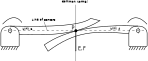
\includegraphics[width=0.8\linewidth]{fig/kennedy_rolling}
   \caption{By Kennedy's Theorem, and shown in Figure \ref{fig:kennedy_sliding}, the instant center of two links in contact lies on the intersection of the common normal and the line of centers. Only if the intersection point \textit{P} lies along the line of centers are the links rolling without sliding. That is, each point \textit{P} on link 2 and link 4 have equal motion along the same line, shown by vectors \textit{E} and \textit{F}.
   This figure was adapted from \cite{ref:kinematics_and_dynamics}}
   \label{fig:kennedy_rolling}.
\end{figure}

Using these definitions, the relationship between \textit{M} and \textit{L} can be derived for a single-stage cycloid. In the case of the single-stage cycloid, there is no motion of point \textit{P} on the housing roller, as it is part of the fixed frame. Therefore, the only relative velocity between the two links comes with the rotation about the instant center between the cycloid plate and housing roller. This can be calculated simply for each pin using the length from the instant center to the contact point, \textit{l\textsubscript{c}}, and the rotational velocity of the cycloid plate, \textit{\textomega\textsubscript{3}}. To calculate the values for pin \textit{i} in the housing, the value \textit{offset} is inserted into the equations.  

\begin{equation} \label{eq:single_slide_offset}
offset = i \frac{2\pi}{N_1}
\end{equation}
\begin{dmath} \label{eq:single_slide_length}
l_{ci} = \bigg\{\left[R-R_r\cos\psi - E N_1 \cos(\phi_2 - offset)\right]^2 
+\\ \left[-R_r \sin{\psi} + E N_1 \sin(\phi_2 - offset)\right]^2 \bigg\}^{1/2}
\end{dmath}
\begin{equation} \label{eq:single_slide_vel}
V_i = \omega_3 * l_{ci}
\end{equation}

Using this relationship, the sliding velocity between the cycloid plate and housing rollers can be determined. However, the cycloid is designed such that the pins rest in the housing and are free to rotate; therefore, the sliding velocity will be translated to a rotational velocity of the pin. An example of the relative sliding velocities for four different input angles, \textphi\textsubscript{2}, can be seen in Figure \ref{fig:single_sliding} with an input velocity, \textomega\textsubscript{2}, of 1.5 rad/s.

\begin{figure}[t]
   \centering
   \begin{tabular}{cc}
	   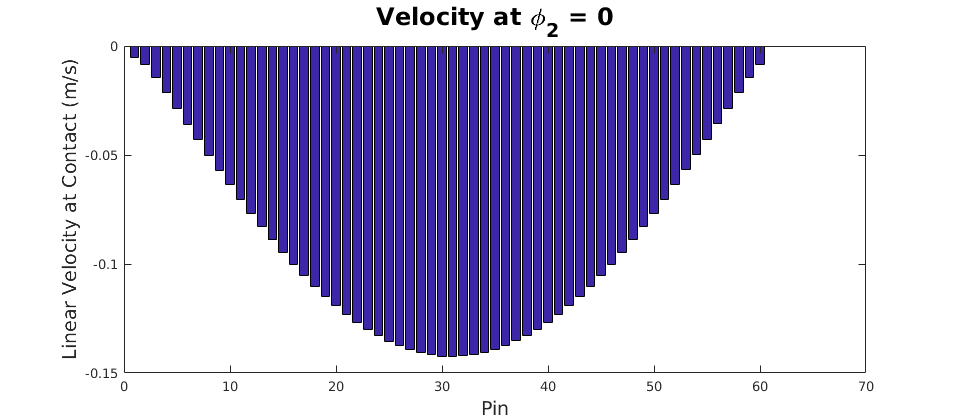
\includegraphics[width=0.48\linewidth]{fig/single_vel_0pi} &
	   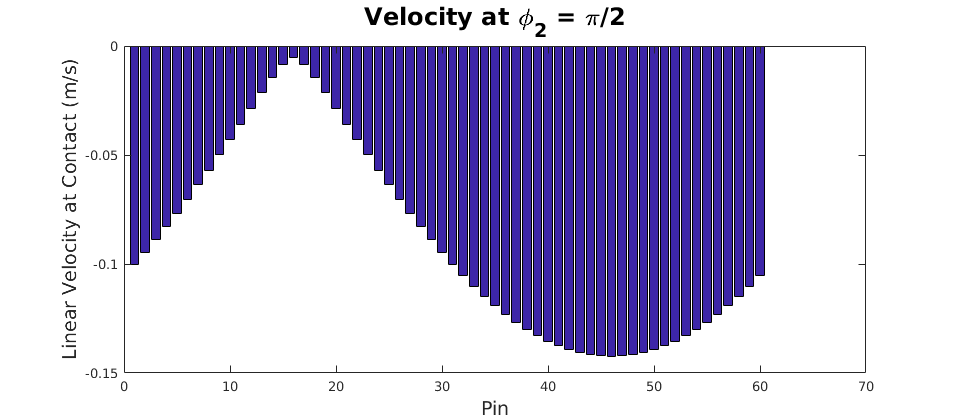
\includegraphics[width=0.48\linewidth]{fig/single_vel_pi_2} \\
	   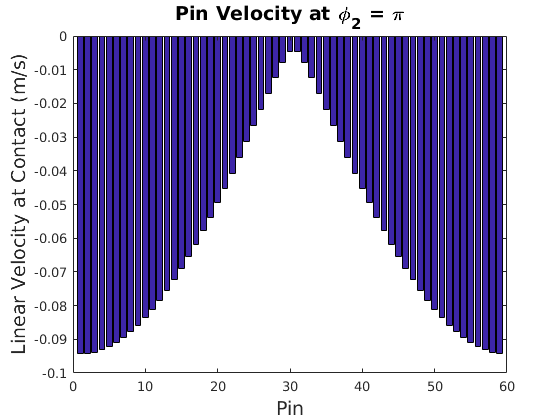
\includegraphics[width=0.48\linewidth]{fig/single_vel_pi} &
	   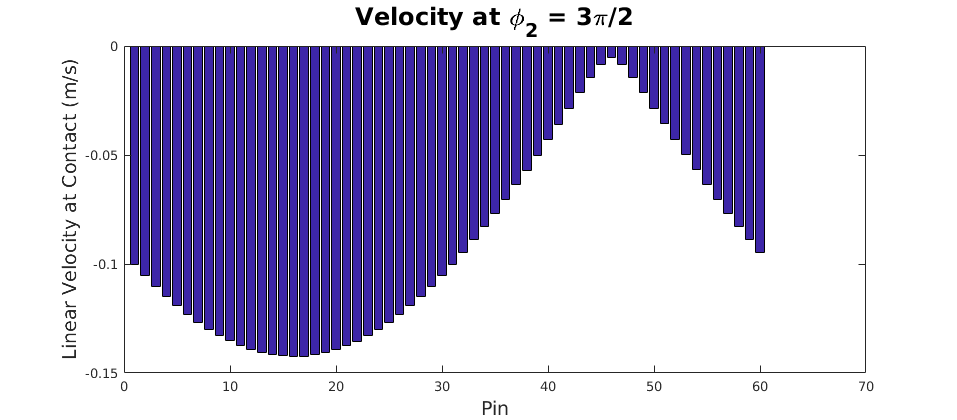
\includegraphics[width=0.48\linewidth]{fig/single_vel_3pi2}
   \end{tabular}
   \caption{Linear velocity at the edge of each pin in the single-stage cycloid through one input rotation with a desired velocity of 1 rad/s.}
   \label{fig:single_sliding}
\end{figure}

\subsection{Predicted Single-Stage Roller Losses} \label{ch:design:pin_roll_1s:predicted_losses}

Due to the assertion that there is sliding of some type (either the plate along the pin or the pin rolling in the housing) and there are forces acting on these pins shown in Figure \ref{fig:single_forces} (discussed in detail in Section \ref{ch:design:single}), there is some loss associated with this interaction that has not previously been captured in the literature. Using the forces developed along the pins in Section \ref{ch:design:single:force_analysis} and the sliding velocities for each pin developed in Section \ref{ch:design:pin_roll_1s:sliding_equations}, the power losses for the system can be estimated using 

\begin{equation} \label{eq:single_power_loss}
P_L = \sum_{i=1}^{N_{1c}}\mu F_{1i} V_i.
\end{equation}
where \textit{N\textsubscript{1c}} is the number of housing pins, \textit{F\textsubscript{1i}} is the force on pin \textit{i} and \textit{V\textsubscript{i}} is the velocity of the interaction at pin \textit{i}.

Note that there will only be losses on pins that have a contact force, which is defined as the number of pins divided by two at any given time. The estimated losses due to the cycloid disk rolling along the housing pins which must then slide in the housing can be calculated for the single-stage cycloid for a given range of inputs. The resulting velocities (Figure \ref{fig:single_sliding}), forces (Figure \ref{fig:single_forces}), and losses (Figure \ref{fig:single_losses}) through one revolution can be observed. Using these calculations, the coefficient of friction can be varied to give an estimate of losses versus coefficient of friction, presented in Figure \ref{fig:single_stage_losses}.

\begin{figure}[!b]
   \centering
   \begin{tabular}{cc}
	   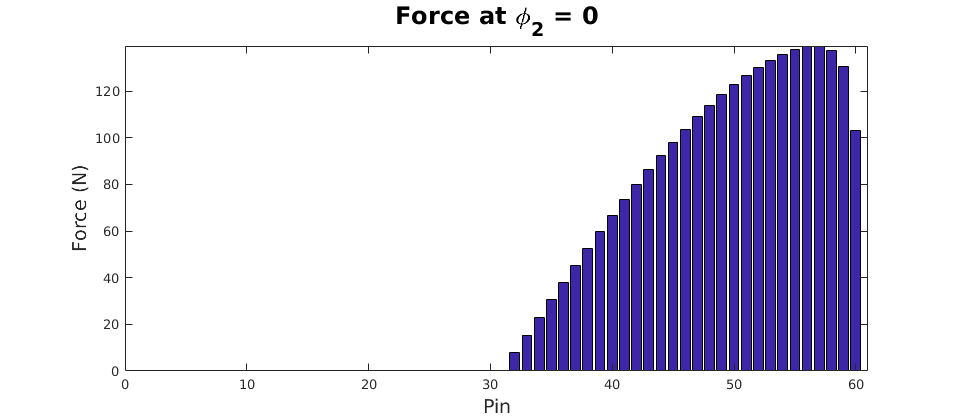
\includegraphics[width=0.48\linewidth]{fig/single_force_0} &
	   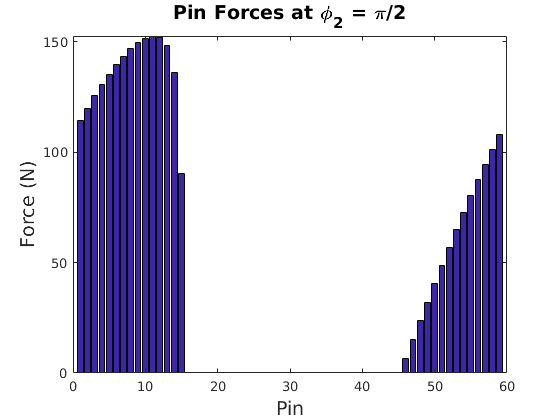
\includegraphics[width=0.48\linewidth]{fig/single_force_pi_2} \\
	   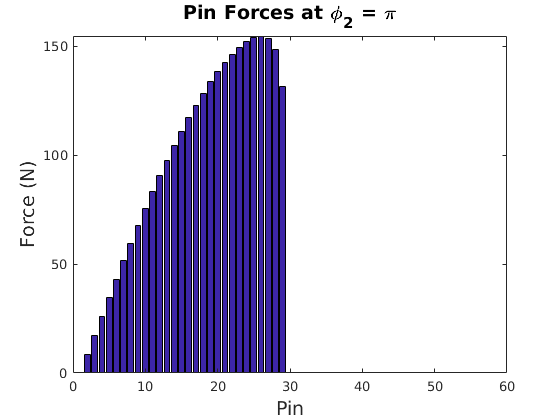
\includegraphics[width=0.48\linewidth]{fig/single_force_pi} &
	   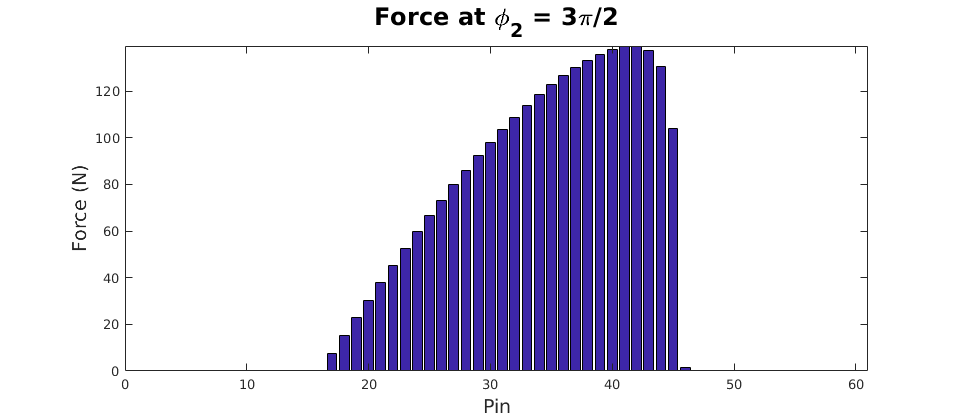
\includegraphics[width=0.48\linewidth]{fig/single_force_3pi2}
   \end{tabular}
   \caption{Forces on each of the pins in the single-stage cycloid through one rotation with a desired output of 100Nm}
   \label{fig:single_forces}
\end{figure}

\begin{figure}[t]
   \centering
   \begin{tabular}{cc}
	   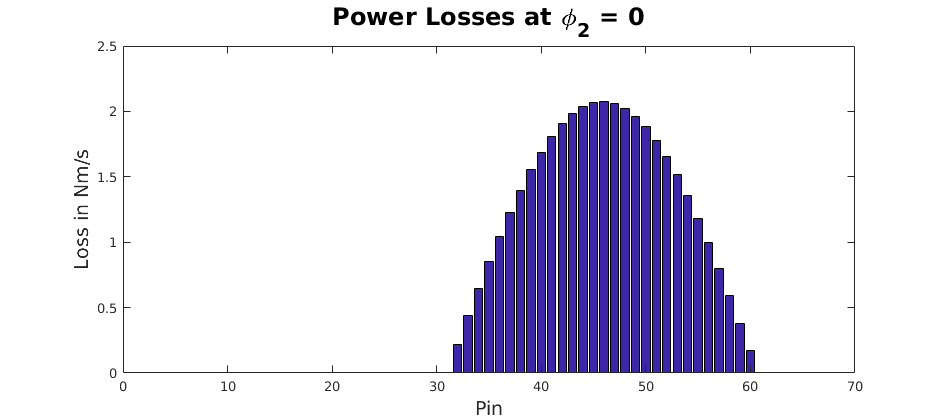
\includegraphics[width=0.48\linewidth]{fig/single_power_0} &
	   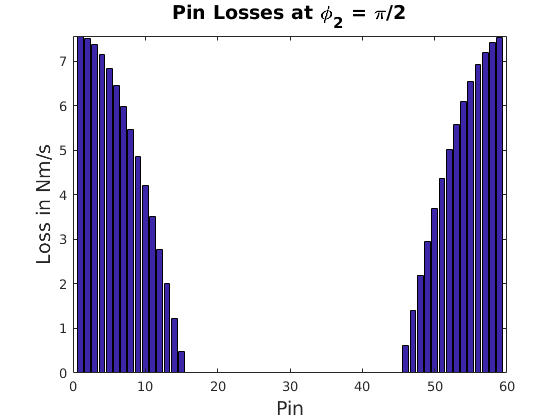
\includegraphics[width=0.48\linewidth]{fig/single_power_pi2} \\
	   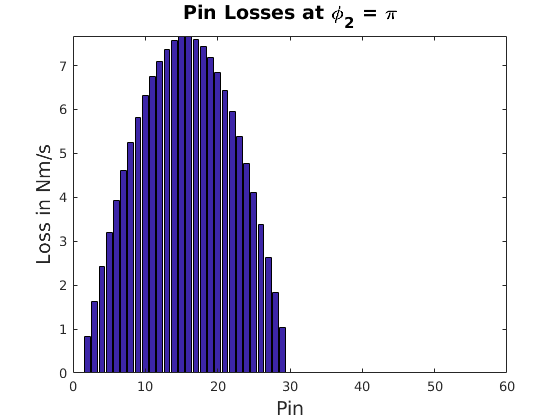
\includegraphics[width=0.48\linewidth]{fig/single_power_pi} &
	   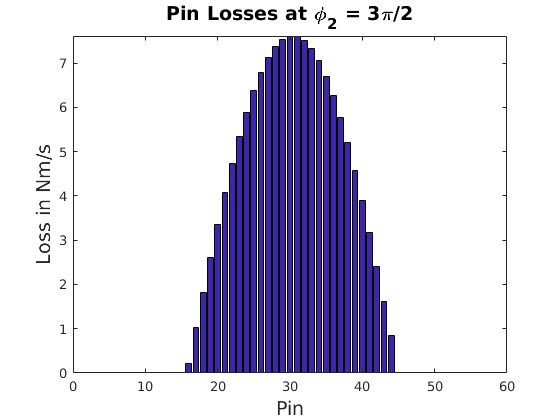
\includegraphics[width=0.48\linewidth]{fig/single_power_3pi2}
   \end{tabular}
   \caption{Losses contributed by the interaction with each housing roller in the single-stage cycloid through a single rotation with a coefficient of friction of 0.03, the best estimate for lubricated steel on steel sliding.}
   \label{fig:single_losses}
\end{figure}

\begin{figure}[t]
	\centering
	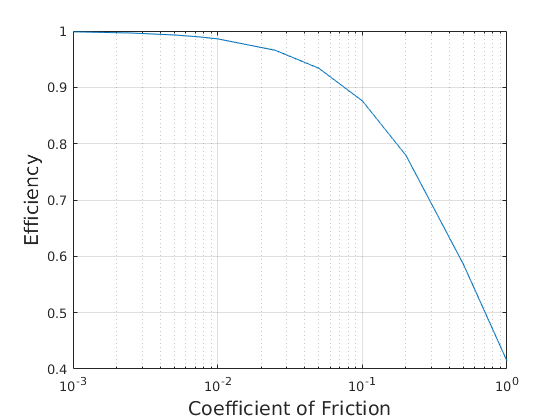
\includegraphics[width=0.75\linewidth]{fig/single_stage_loss}
   \caption{Losses contributed by the lobe to pin interaction for a range of coefficients of friction. This does not include losses from other interactions such as the output rollers or input bearings.}
   \label{fig:single_stage_losses}
\end{figure}



The losses of each pin can be summed to get the instantaneous power loss of the cycloid due to the interaction between the cycloid plate and the housing pins. Due to the direct scaling of force per pin and velocity per pin with input force and velocity, the input values do not affect the predicted efficiency for a given input of \textmu. However, there are other losses present in the system, such as the input bearing, resulting in losses that scale with torque shown in Chapter \ref{ch:single}. Figure \ref{fig:single_stage_losses} shows the predicted losses for the constructed single-stage. Generally, the losses for lubricated steel on steel range from 0.03 to 0.15. If the minimum of that is used, the losses due only to the interaction of the pins and lobes for this design is 95\%, not including any other losses. This does suggest that relatively high efficiencies, over 90\%, can be achieved with realistic coefficients of friction that could be expected, giving validity to an efficient high reduction, pin-in-housing design. 

\section{Single-Stage Design} \label{ch:design:single}
% Talk about items that are specific to a single-stage design, specifically the load calculations and such to size the plates and the disks 

After the development of the basic equations for the profile of the cycloid, the practical design considerations must take place to allow for the desired loads and reduction to be carried through the cycloid for the given application. These application-specific design values will be discussed briefly as they pertain to the literature. This actuator was originally designed by robotics engineers at NASA: Johnson Space Center. The design equations used are presented to lay the foundation for the analysis and the testing results contributed by this thesis.

\subsection{Single-Stage Cycloid Design Requirements}

In 2007 and 2008, NASA developed a manned rover prototype for planetary surfaces for future missions \cite{ref:rover}.
This robotic vehicle is made up of six independent wheel modules, each with their own drive, steering, and both active and passive suspension.
In 2014, a new prototype wheel module was designed and created to analyze potential technologies that could be used in these applications.
In the new design layout, it was possible for the drive wheels to counter-rotate against the steering and put large shock loads into the steering system.
These requirements which called for a compact package, high load, high shock load, and allowed tolerance of backlash and lent themselves to the selection of a cycloidal drive for the steering actuator.
The prototype wheel module layout can be seen in Figure \ref{fig:wheel_module}.

\begin{figure}[!b]
   \centering
   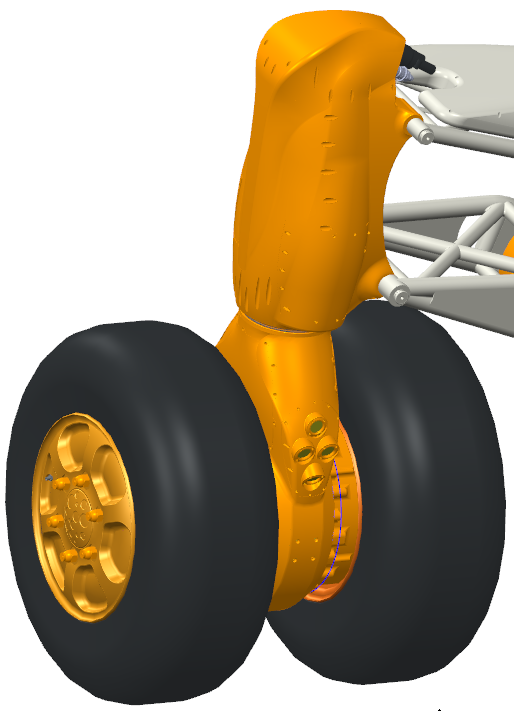
\includegraphics[width=0.40\linewidth]{fig/wheel_module_CAD}
   \caption{CAD model of rover wheel module prototype.
   Suspension arms hold the steering column.
   Each wheel has an in-wheel drive motor.}
   \label{fig:wheel_module}
\end{figure}

\begin{table*}[t]
  \vskip0.2cm
  \caption{Designed Duty Cycles for System}
  \label{table:duty_cycle}
  \begin{center}
    \vskip-0.2cm
    \begin{tabular}{|p{0.10\textwidth}||p{0.15\textwidth}||p{0.15\textwidth}| |p{0.15\textwidth}| |p{0.15\textwidth}|}
    \hline
    Time Used & Output Torque (Nm) & Output Speed (RPM) & Actuator Torque (Nm) & Actuator Speed (RPM)\\
    \hline
    5\% & 2440 & 6.8 & 554.7 & 33.9\\
    \hline
    20\% & 1627 & 6.8 & 369.8 & 33.9\\
    \hline
    60\% & 542 & 15.3 & 123.3 & 76.3\\
    \hline
    15\% & 135 & 15.3 & 30.8 & 76.3\\
    \hline
    \end{tabular}
  \end{center}
\end{table*}

Based on the load cases, the actuator was required to output a stall torque of 2,440 Nm (1800 ft-lb) with a maximum output speed of 1.57 rad/s (90 deg/s) at 1,626 Nm (1200 ft-lb).
The required torque/speed data points are presented in Table \ref{table:duty_cycle} with an assumed loss of 88\% chosen based on the available literature.
The actuator layout for the vehicle placed the motor and cycloid off center of the steering axis with an additional 5:1 reduction into the steering column, thus decreasing the torque needed for the cycloid output but increasing the potential shock loading.

\subsection{Force Analysis and Sizing} \label{ch:design:single:force_analysis}

First, the motor and cycloid reduction were sized together to determine the appropriate motor and reduction to use for the system. The motor used was a Parker Frameless Kit Motor, model K089200-7Y, with no hall commutation. This was used in conjunction with a cycloid reduction of 59:1 which was mounted to a final 5:1 reduction to the steering output. The motor is commutated using a Renishaw RM-44 magnetic encoder mounted to the input shaft. 

Knowing the final reduction and the necessary output torque, the maximum load developed by the cycloid (\textit{F\textsubscript{max}}) is 488 Nm, and the maximum speed of the cycloid, \textomega\textsubscript{max}, is 7.85 rad/s. These values can be used in conjunction with a well defined set of equations presented in previous works \cite{ref:malhorta_2}, \cite{ref:li}, and \cite{ref:unified_approach} to determine the allowable sizes of the components of the system. The analysis presented by Malhorta and Parameswaran details the equations necessary for calculating the loads on the housing pins and the output pins for a single-stage design. This methodology has been adopted for this work and will be further expanded upon in Chapter \ref{ch:dual}, so it is presented in its completeness here. 

\begin{figure}[t]
   \centering
   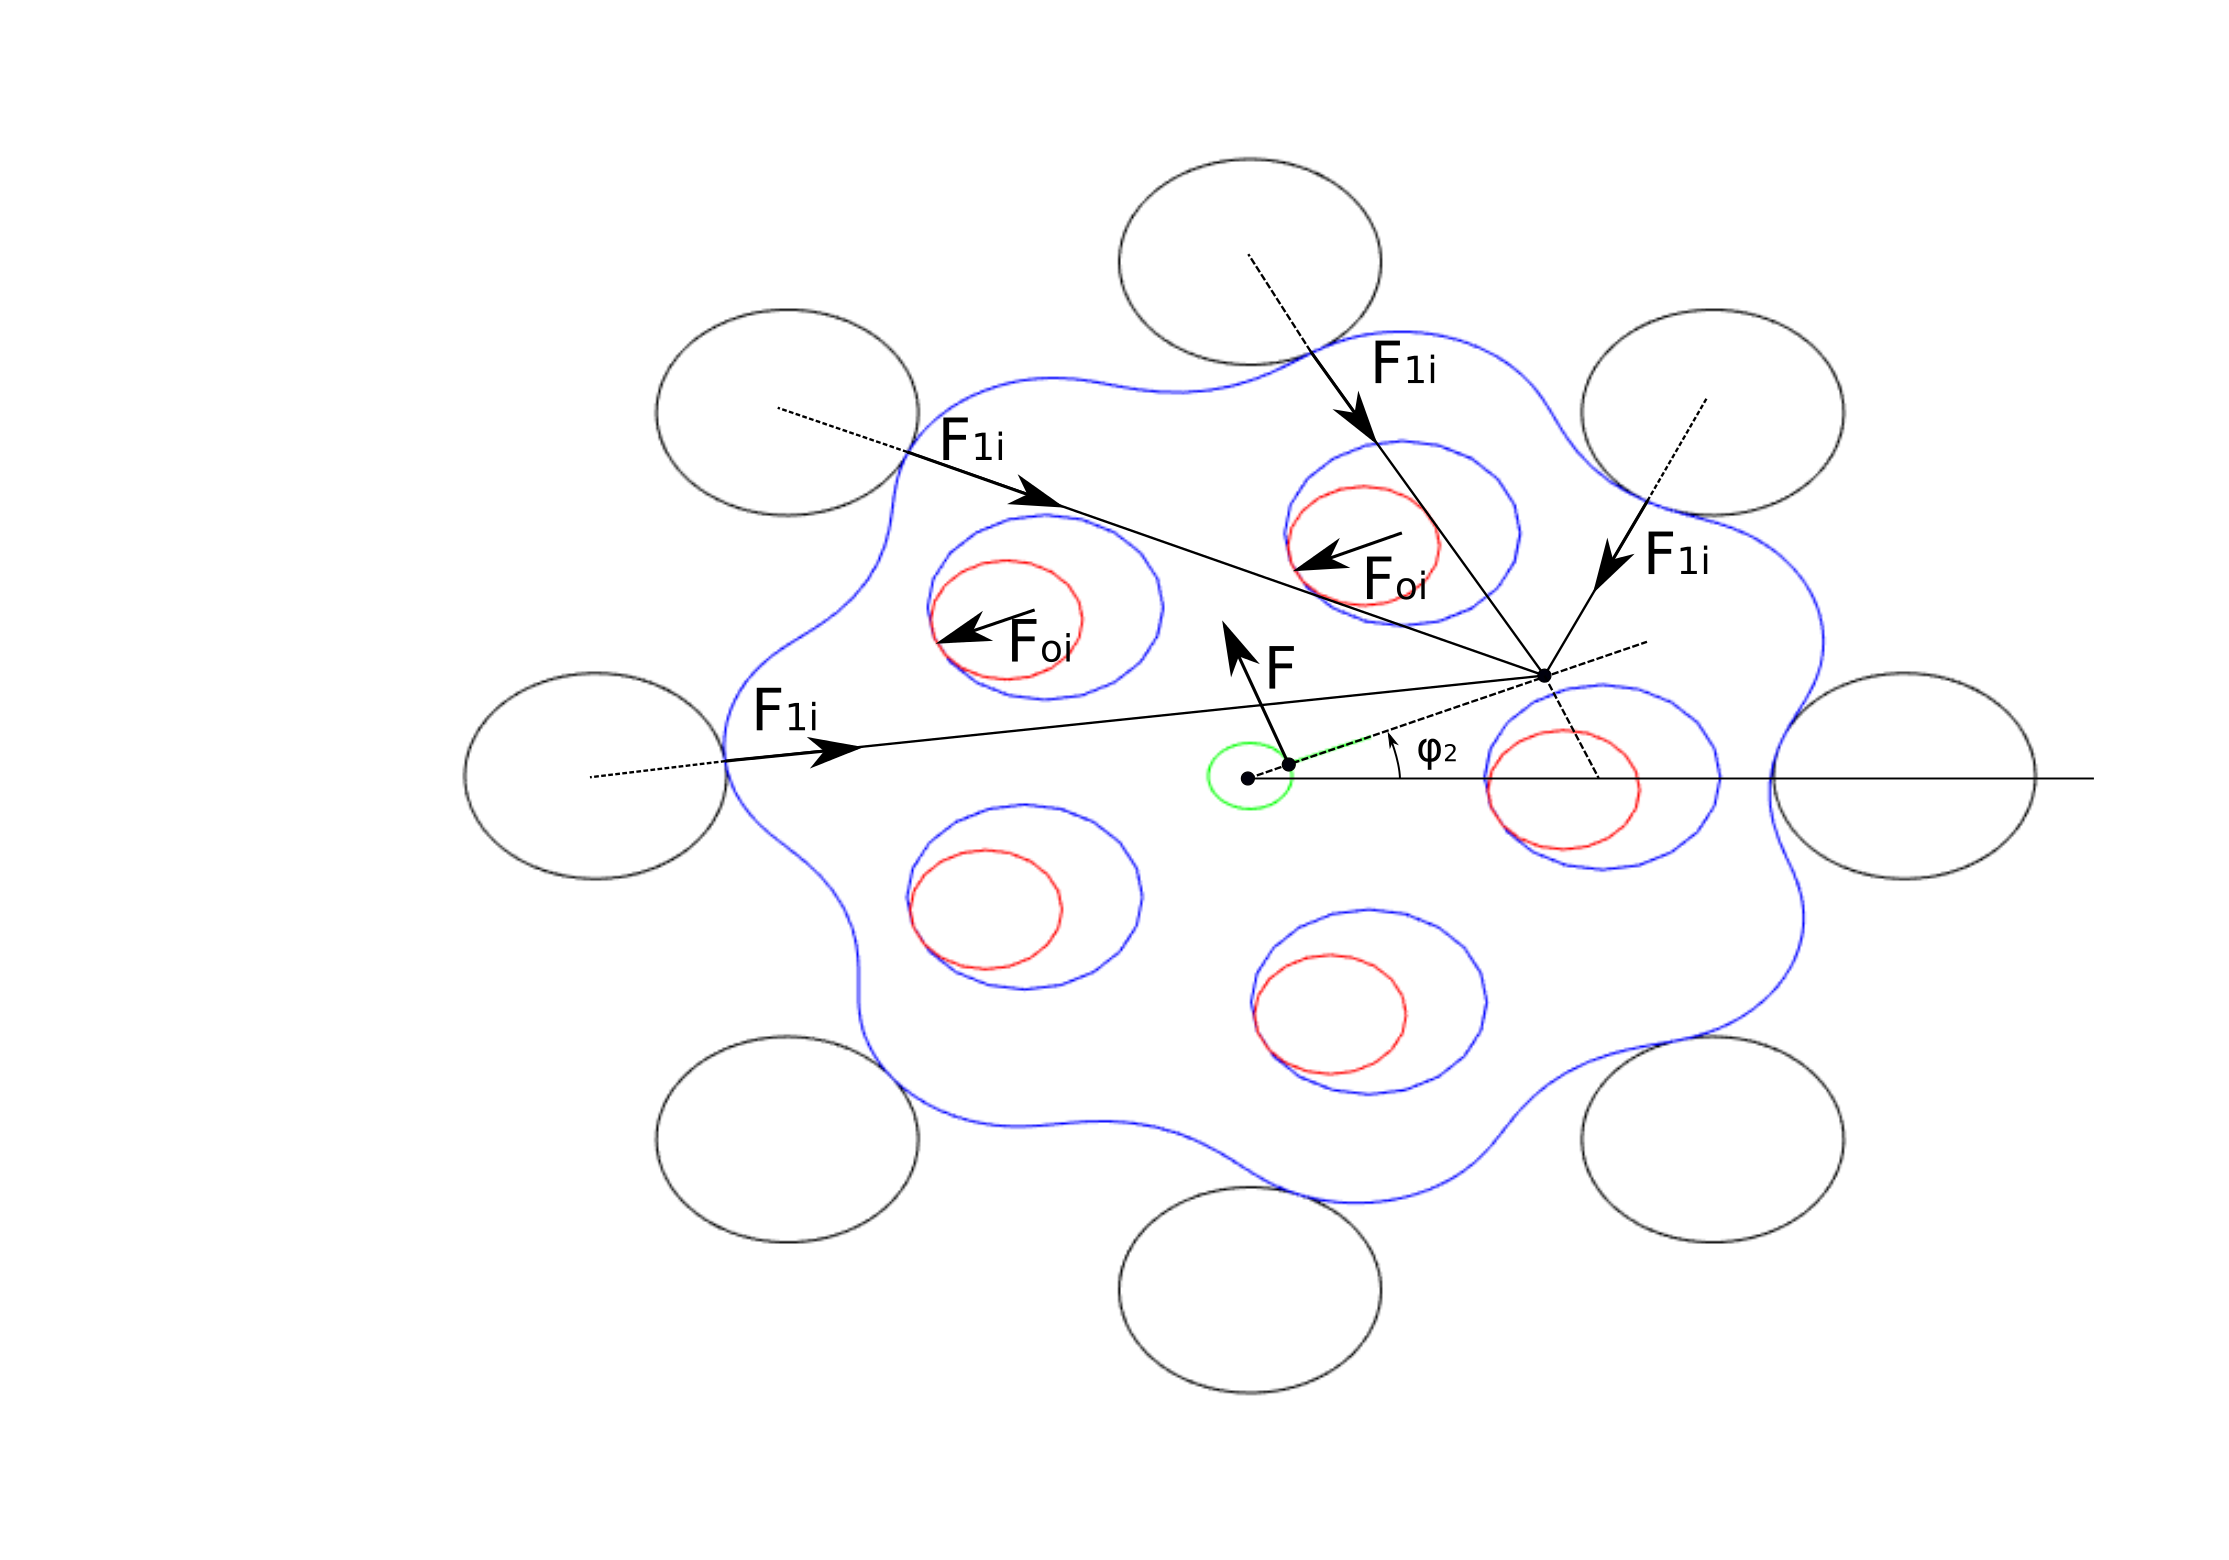
\includegraphics[width=01.0\linewidth]{fig/single_loads}
   \caption{Loads present in a single stage cycloid.}
   \label{fig:single_loads}
\end{figure}

The interaction between the elements of a single-stage cycloid can be seen in Figure \ref{fig:single_loads} that details the forces present in a cycloid. The input force from the motor drives through the eccentric bearing to the cycloid plate. These loads are then reacted through the housing rollers and output pins. One will notice that the loads can only form on half of the rollers and pins at a time, as these members are in compression, and if a tension force forms, they will separate and not carry load. In a perfectly manufactured arrangement, the number of lobes in contact, \textit{N\textsubscript{lc}}, and output pins in contact, \textit{N\textsubscript{oc}}, is simply 


\begin{equation}
N_{1c} = \frac{N_{1} - 1}{2},\ if\ (N_1 -1)\ is\ even 
\end{equation}
\begin{equation}
= \frac{(N_{1}-1) - 1}{2},\ if\ (N_{1} - 1)\ is\ odd 
\end{equation}
\begin{equation}
N_{oc} = \frac{N_{pins}}{2},\ if\ N_{pins}\ is\ even 
\end{equation}
\begin{equation}
= \frac{N_{pins} - 1}{2},\ if\ N_{pins}\ is\ odd 
\end{equation}

There geometric values are depicted in Figure \ref{fig:single_loads_angles} that must be defined in order to successfully calculate the loads in the next step. These are written simply in \cite{ref:hwang_geometry} and are shown below in Equations \ref{eq:single_b} -- \ref{eq:single_l} for each housing pin \textit{i}. 

\begin{figure}[!b]
   \centering
   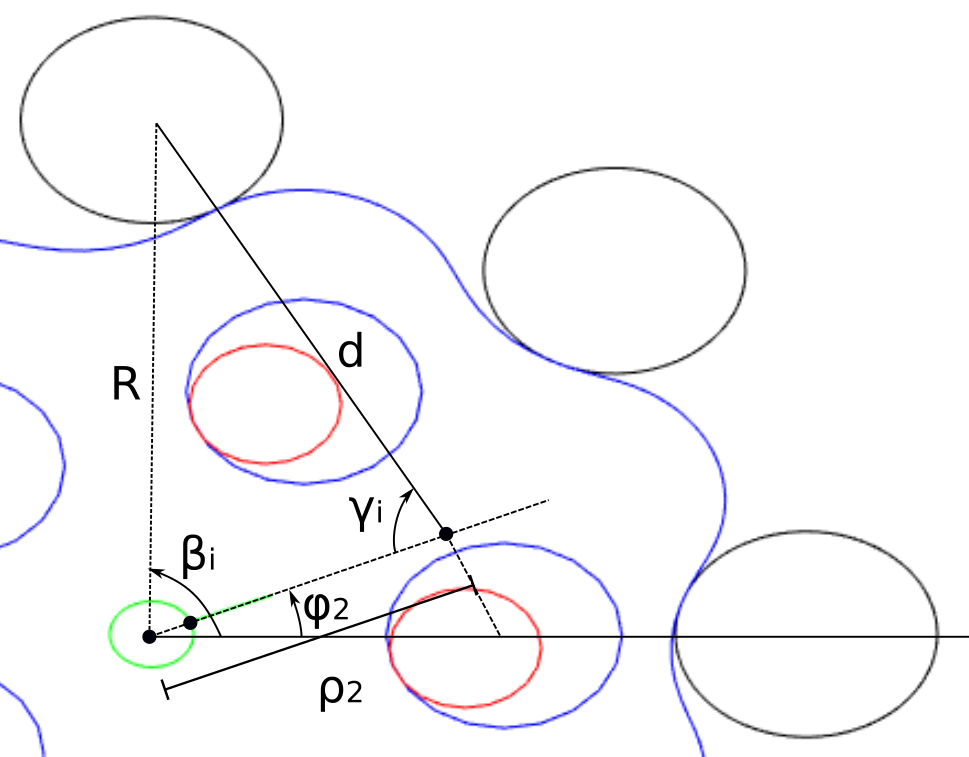
\includegraphics[width=0.6\linewidth]{fig/single_loads_angles}
   \caption{Necessary angles required to calculate the loads at each individual housing pin for a single-stage cycloid.}
   \label{fig:single_loads_angles}
\end{figure}

\begin{equation} \label{eq:single_b}
\beta_i = \frac{2\pi i}{N_1}
\end{equation}
\begin{equation} \label{eq:single_d_x}
d_x = R \cos(\beta_i) - E N_1 \cos(\phi_2)
\end{equation}
\begin{equation} \label{eq:single_d_y}
d_y = R\sin(\beta_i) - E N_1 \sin(\phi_2)
\end{equation}
\begin{equation} \label{eq:single_d}
d = \sqrt{d_x^2 + d_y^2}
\end{equation}
\begin{equation} \label{eq:single_gamma}
\gamma_i = \sin^{-1}\left[{\frac{R \sin{\beta_i - \phi_2}}{d}}\right]
\end{equation}
\begin{equation} \label{eq:single_rho2}
\rho_2 = \rho_1 - E
\end{equation}
\begin{equation} \label{eq:single_l}
l_i = \rho_2 \sin{\gamma_i}
\end{equation}

Using this knowledge, the forces on the contacting lobes and pins can be calculated. This calculation methodology starts with a power analysis to determine the forces on the output pins (Eq. \ref{eq:single_power}). Using this as a basis, equations for the forces in the x-direction (Eq. \ref{eq:single_x}), y-direction (Eq. \ref{eq:single_y}), and the moment about the cycloid plate's center (Eq. \ref{eq:single_torque}) can be written for any reducer with \textit{N\textsubscript{c1}} lobes (\textit{N\textsubscript{1}} housing rollers) and \textit{N\textsubscript{p1}} output pins. The force on housing roller \textit{i} is denoted as \textit{F\textsubscript{ri}} and on output pin \textit{j} as \textit{F\textsubscript{oj}}.

\begin{equation} \label{eq:single_power}
M_a = \frac{R_o}{N_1} \sum_{j=1}^{N_{oc}} F_{oj} \sin(\beta_j + N_1 \phi_2)
\end{equation}
\begin{equation} \label{eq:single_x}
\sum_{i=1}^{N_{1c}} F_{ri} \cos{\alpha_i} - \sum_{j=1}^{N_{oc}} F_{oj} \cos(N_1*\phi_2) - F_{input} \sin{\gamma} = 0
\end{equation}
\begin{equation} \label{eq:single_y}
-\sum_{i=1}^{N_{1c}} F_{ri} sin{\alpha_i} + \sum_{j=1}^{N_{oc}} F_{oj} sin(N_1*\phi_2) + F_{input} \cos{\gamma} = 0
\end{equation}
\begin{equation} \label{eq:single_torque}
\sum_{i=1}^{N_{1c}}F_{ri} l_i - \sum_{j=1}^{N_{oc}}F_{oj} R_o \sin(\beta_j + N_1 \phi_2) = 0
\end{equation}

In order to solve this system of equations, an additional assumption must be made, that is, that the forces on the pins and rollers are relative to their length \textit{l\textsubscript{ij}}.

\begin{equation} 
\frac{F_{1i}}{l_{1i}} = constant 
\end{equation}
\begin{equation}
\frac{F_{oi}}{l_{oi}} = constant
\end{equation}

Using this system of equations, the forces on the input pins can be determined for a given cycloid system. However, these equations assume that the forces are being shared perfectly across all lobes and pins that could be in contact at any given time. Due to the nature of real life and manufacturing tolerances, fewer than the ideal number of pins will be in contact. Therefore, the pins should be sized such that if a single pin takes this force, it will not fail, and it can be assumed that the plate would deform such that additional pins and lobes would begin to take the load. Using these assumptions, the maximum loads on a single lobe and output roller for the designed cycloid are shown in Table \ref{table:single_loads}, which leads to the necessary sizing of components in Table \ref{table:single_sizing}.

\begin{table}
  \vskip0.2cm
  \caption{Single-Stage Calculated Loads}
  \label{table:single_loads}
  \begin{center}
    \vskip-0.2cm
    \begin{tabular}{|c|c|}
    \hline
  Variable & Value\\
  \hline
  \textit{F\textsubscript{roller}} & 11 kN\\
  \hline
  \textit{\textsigma\textsubscript{roller}} & 643 kPa\\
  \hline
  \textit{F\textsubscript{output-pin}} & 14.8 kN\\
  \hline
  \textit{\textsigma\textsubscript{output-pin}} & 722 kPa\\
  \hline
    \end{tabular}
  \end{center}
\end{table}

\begin{table}
  \vskip0.2cm
  \caption{Single-Stage Design Values}
  \label{table:single_sizing}
  \begin{center}
    \vskip-0.2cm
    \begin{tabular}{|c|c|}
    \hline
  Design Variable & Value\\
  \hline
  \textit{N\textsubscript{lobes}} & 59\\
  \hline
  \textit{N\textsubscript{rollers}} & 60\\
  \hline
  \textit{Eccentricity} & 0.762 mm\\
  \hline
  \textit{Roller Offset Radius} & 50.8 mm\\
  \hline
  \textit{Housing Roller Radius} & 1.58 mm\\
  \hline
  \textit{Cycloid Plate Thickness} & 7.94 mm\\
  \hline
  \textit{Cycloid Plate Material} & 17-4 PH Stainless Steel\\
  \hline
  \textit{Housing Roller Material} & Stainless Steel\\
  \hline
  \textit{Output Pin Material} & Stainless Steel \\
  \hline
    \end{tabular}
  \end{center}
\end{table}

\subsection{Final Single-Stage Design} \label{ch:design:single:final}

Using the equations and analysis laid out in Section \ref{ch:design:basic_calc:overview} and Section \ref{ch:design:single:force_analysis}, the final design was completed and manufactured. In the design, the cycloid plates need a thickness of 7.94 mm. To accomplish this thickness and balance the system for vibrations, three cycloid plates are used in tandem, each 120$^\circ$ offset from the others. In this design, the housing rollers are free to rotate. A channel is cut into the housing, and the pin rests in that channel, so it is assumed they will slide freely. The output pins, however, are pressed into the output plate, so they are assumed to remain fixed through operation, and this assumption is validated in the results. The cross section profile of the CAD model can be seen in Figure \ref{fig:single_stage}.

\begin{figure}[!b]
   \centering
   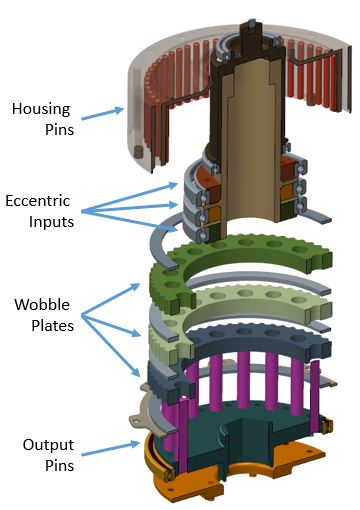
\includegraphics[width=0.5\linewidth]{fig/exploded_labeled}
   \caption{Exploded view of the cycloidal reducer.
   Three cycloid plates are driven by the input shaft with 120$^\circ$ offsets.
   The ring pins are free pins inserted in the housing.
   The output has pins run through all three cycloid plates to harness the counter-rotation for the drive output.}
   \label{fig:single_stage}
\end{figure}

